\documentclass[11pt,a4paper]{article}
\usepackage[utf8]{inputenc}
\usepackage{geometry}
\geometry{top=0.85in, bottom=0.85in, left=0.9in, right=0.9in}
\usepackage{amsmath,amssymb,amsfonts}
\usepackage{graphicx}
\usepackage{hyperref}
\usepackage{booktabs}
\usepackage{array}
\usepackage{tabularx}
\usepackage{xcolor}
\usepackage{float}
\usepackage{enumitem}
\usepackage{abstract}
\usepackage{titlesec}
\usepackage{tikz}
\usetikzlibrary{shapes.geometric, arrows.meta, positioning, shadows, calc, backgrounds}

% Professional Color Palette
\definecolor{primary}{RGB}{30, 41, 59}       % Slate Dark
\definecolor{secondary}{RGB}{15, 118, 110}   % Teal Deep
\definecolor{accent}{RGB}{225, 29, 72}       % Rose Red
\definecolor{warning}{RGB}{234, 88, 12}      % Amber Orange
\definecolor{safe}{RGB}{22, 163, 74}         % Emerald Green
\definecolor{lightbg}{RGB}{248, 250, 252}    % Soft Gray

% Hyperlink Configuration
\hypersetup{
    colorlinks=true,
    linkcolor=secondary,
    citecolor=secondary,
    urlcolor=secondary
}

% Section Title Formatting
\titleformat{\section}{\Large\bfseries\color{primary}}{\thesection}{1em}{}
\titleformat{\subsection}{\large\bfseries\color{secondary}}{\thesubsection}{1em}{}
\titleformat{\subsubsection}{\bfseries\color{primary}}{\thesubsubsection}{1em}{}

% Title and Formatted Author Block
\title{\vspace{-0.6cm}\Large\bfseries SmokeGuard AI: A Real-Time Dual-YOLO Cigarette Smoking Violation Detection and Spatial Containment Analytics Platform}

\author{
    \textbf{Tarun Kumar Agnihotri}\textsuperscript{1,*}, \quad 
    \textbf{Arnav Singh}\textsuperscript{2}, \quad 
    \textbf{Shubh Jaiswal}\textsuperscript{2} \\[0.5em]
    \small \textsuperscript{1}\textbf{Lead Author \& Technical Architect}: System Engineering, Full-Stack \& ML Development \\
    \small \textsuperscript{2}\textbf{Co-Authors \& Research Analysts}: Literature Survey, Research Gap \& Theoretical Formulation \\[0.3em]
    \small Department of Computer Science \& Artificial Intelligence \\
    \small \texttt{*tarunagnihotri534@gmail.com}
}

\date{\today}

\begin{document}

\maketitle

\renewcommand{\abstractname}{\vspace{-0.5cm}Abstract}
\begin{abstract}
\noindent Automated monitoring of cigarette smoking in non-smoking facilities is essential for public health, structural fire safety, and regulatory compliance. Traditional computer vision prototypes suffer from high false-alarm rates caused by extreme bounding box scale mismatches, temporal detection flickering, and prohibitive network bandwidth consumption when streaming processed video feeds. This paper presents \textbf{SmokeGuard AI}, a full-stack real-time smoking violation detection platform. The system leverages dual-YOLO model inference (\texttt{yolo11s} for person tracking via ByteTrack and a specialized \texttt{best.pt} model for cigarette identification), a novel Spatial Containment Ratio algorithm ($\mathcal{C} \ge 0.30$) to accurately link micro-bounding boxes, a 5-frame debounced state machine to eliminate false alarms, and a low-bandwidth WebSocket JSON telemetry pipeline with client-side HTML5 Live Canvas rendering. Complete functional requirements, non-functional constraints, hardware/software specifications, and modular flowcharts are formally documented.
\\[0.3em]
\textbf{Keywords:} Computer Vision, YOLOv11, ByteTrack Multi-Object Tracking, Spatial Containment, Real-Time Analytics, WebSockets, FastAPI.
\end{abstract}

\hrule \vspace{0.8em}

\section{Introduction}

Automated video analytics in modern facility surveillance play a vital role in enforcing safety and compliance regulations. Detecting cigarette smoking via computer vision presents unique technical challenges: cigarettes occupy a minimal fraction of total pixel area, undergo rapid spatial motion near the human face, and are subject to frequent hand and facial occlusions. Furthermore, benign objects such as pens, straws, or fingers brought near the mouth frequently trigger false positives in single-frame visual detectors.

\textbf{SmokeGuard AI} is an enterprise-grade platform engineered to address these challenges through a unified multi-stage architecture:
\begin{enumerate}[leftmargin=*]
    \item \textbf{Dual-Model Computer Vision Pipeline}: Executes parallel inference using a COCO-pretrained \texttt{yolo11s.pt} model for person detection coupled with ByteTrack persistent track ID assignment, alongside a custom-trained \texttt{best.pt} model optimized for small-object cigarette detection.
    \item \textbf{Spatial Containment Linking Algorithm}: Replaces standard Intersection over Union (IoU) with a Spatial Containment Ratio ($\mathcal{C} \ge 0.30$) that measures what fraction of the small cigarette bounding box lies inside the human bounding box envelope.
    \item \textbf{Debounced Temporal State Machine}: Filters out visual flickering by requiring $N=5$ consecutive smoking-associated frames before escalating a person's status from candidate `"smoking"` to confirmed `"violation"`.
    \item \textbf{Decoupled Low-Bandwidth Telemetry}: Pushes lightweight JSON coordinate event payloads over WebSockets (\texttt{ws://localhost:8000/ws/live}) alongside an MJPEG video feed, allowing the Next.js 14 frontend to render interactive vector bounding boxes client-side without heavy server-side video re-encoding.
    \item \textbf{Automated Forensic Audit Pipeline}: Automatically logs snapshot evidence and metadata (\texttt{camera\_id}, \texttt{track\_id}, timestamps, confidence scores) into SQLite/PostgreSQL, with RESTful APIs supporting CSV exports.
\end{enumerate}

\section{Research Gap Analysis}

Automated smoking detection sits at the intersection of small-object detection, multi-object tracking, and operational compliance reporting. A systematic review of traditional detection prototypes reveals five critical technical gaps that SmokeGuard AI explicitly addresses:

\begin{enumerate}[leftmargin=*]
    \item \textbf{Small-Object Association Failure}: Standard IoU ($\frac{|A \cap B|}{|A \cup B|}$) measures overlap relative to the combined union area. Because a cigarette box is tiny compared to a person box, standard IoU approaches zero even when the cigarette is completely inside the person envelope, causing target linking to fail. SmokeGuard AI formulates a Spatial Containment Ratio:
    \begin{equation}
    \mathcal{C}(B_C, B_P) = \frac{\text{Area}(B_C \cap B_P)}{\text{Area}(B_C)} \ge 0.30
    \end{equation}
    Which evaluates what fraction of the small cigarette box lies inside the human envelope, ensuring robust target association regardless of distance.
    
    \item \textbf{Alert Instability from Single-Frame Decisions}: Standard pipelines trigger an alert instantly upon a single positive classification, producing severe false positives from transient hand gestures, pens, or straws. SmokeGuard AI introduces a \textit{Debounced State Machine} requiring $N=5$ consecutive positive frames across persistent ByteTrack IDs before confirming a violation.

    \item \textbf{Bandwidth-Heavy Real-Time Streaming}: Conventional dashboards burn bounding box graphics directly into video frames on the server and stream heavy annotated high-bitrate video streams, choking network bandwidth and GPU resources. SmokeGuard AI decouples video from telemetry, emitting structured coordinate JSON over WebSockets for client-side HTML5 Canvas rendering.

    \item \textbf{Missing Evidence and Audit Trail}: Detection-only prototypes frequently lack persistent evidence logging, real-time database storage, and queryable administrative interfaces. SmokeGuard AI automatically captures JPEG snapshots on state transitions, records metadata in SQLite/PostgreSQL, and exposes REST endpoints for CSV report exports.

    \item \textbf{Lack of Externally Configurable Thresholds}: Most research prototypes utilize hard-coded detection parameters. SmokeGuard AI centralizes all detection, tracking, overlap, and debounce thresholds into a single configuration module (\texttt{ml/inference/config.py}).
\end{enumerate}

\section{System Requirements Analysis}

\subsection{Functional Requirements}

The functional requirements of SmokeGuard AI are enumerated in Table~\ref{tab:functional_reqs}.

\begin{table}[H]
\centering
\caption{Functional Requirements (FR) Matrix}
\label{tab:functional_reqs}
\small
\vspace{0.4em}
\begin{tabularx}{\textwidth}{l X}
\toprule
\textbf{Req ID} & \textbf{Requirement Description} \\
\midrule
\textbf{FR1} & The system shall detect persons in each incoming video frame using \texttt{yolo11s.pt}. \\
\textbf{FR2} & The system shall assign and maintain a persistent track ID for each person using ByteTrack. \\
\textbf{FR3} & The system shall detect cigarettes in each frame using custom-trained \texttt{best.pt}. \\
\textbf{FR4} & The system shall compute a spatial containment ratio to link detected cigarettes to tracked persons. \\
\textbf{FR5} & The system shall require a configurable number of consecutive smoking frames ($N=5$) before confirming a violation. \\
\textbf{FR6} & The system shall broadcast per-frame detection JSON results over WebSockets in real time. \\
\textbf{FR7} & The client dashboard shall render color-coded bounding boxes and labels over the live feed. \\
\textbf{FR8} & The system shall automatically capture a JPEG snapshot at the moment a violation is confirmed. \\
\textbf{FR9} & The system shall persist violation metadata (\texttt{camera\_id}, \texttt{track\_id}, timestamps, confidence) to database. \\
\textbf{FR10} & The system shall expose REST endpoints to start/stop streams, list violations, view stats, and export CSVs. \\
\textbf{FR11} & The system shall accept USB webcam index \texttt{0}, video file paths, or RTSP URLs as stream inputs. \\
\bottomrule
\end{tabularx}
\end{table}

\subsection{Non-Functional Requirements}
\begin{itemize}[leftmargin=*]
    \item \textbf{Real-Time Performance}: Inference and event broadcasting operate with sub-second delay suitable for live surveillance feeds.
    \item \textbf{Low-Bandwidth Transport}: Transmits minimal coordinate telemetry JSON instead of server-rendered annotated JPEGs.
    \item \textbf{Reliability}: Debounced temporal confirmation suppresses transient false alarms.
    \item \textbf{Auditability}: Every violation record is persistently linked to camera source, track ID, timestamps, snapshot evidence, and confidence scores.
    \item \textbf{Portability \& Containerization}: Full stack deployable via Docker and Docker Compose (FastAPI GPU + Postgres + Next.js).
\end{itemize}

\subsection{Hardware and Software Specifications}
\begin{itemize}[leftmargin=*]
    \item \textbf{Hardware Requirements}: NVIDIA GPU-enabled host machine recommended for CUDA acceleration; video input source (Webcam / RTSP IP Camera); persistent storage scaling with violation audit retention.
    \item \textbf{Software Stack}: Python 3.10+, FastAPI, Uvicorn, PyTorch, Ultralytics YOLOv11, ByteTrack, OpenCV, Node.js 18+, Next.js 14, React, TailwindCSS, SQLite / PostgreSQL, Docker Compose.
\end{itemize}

\section{System Architecture and Operational Flowchart}

The operational workflow follows a strict, end-to-end execution path. Figure~\ref{fig:vertical_flowchart} illustrates the vertical execution flowchart of the system.

\begin{figure}[H]
\centering
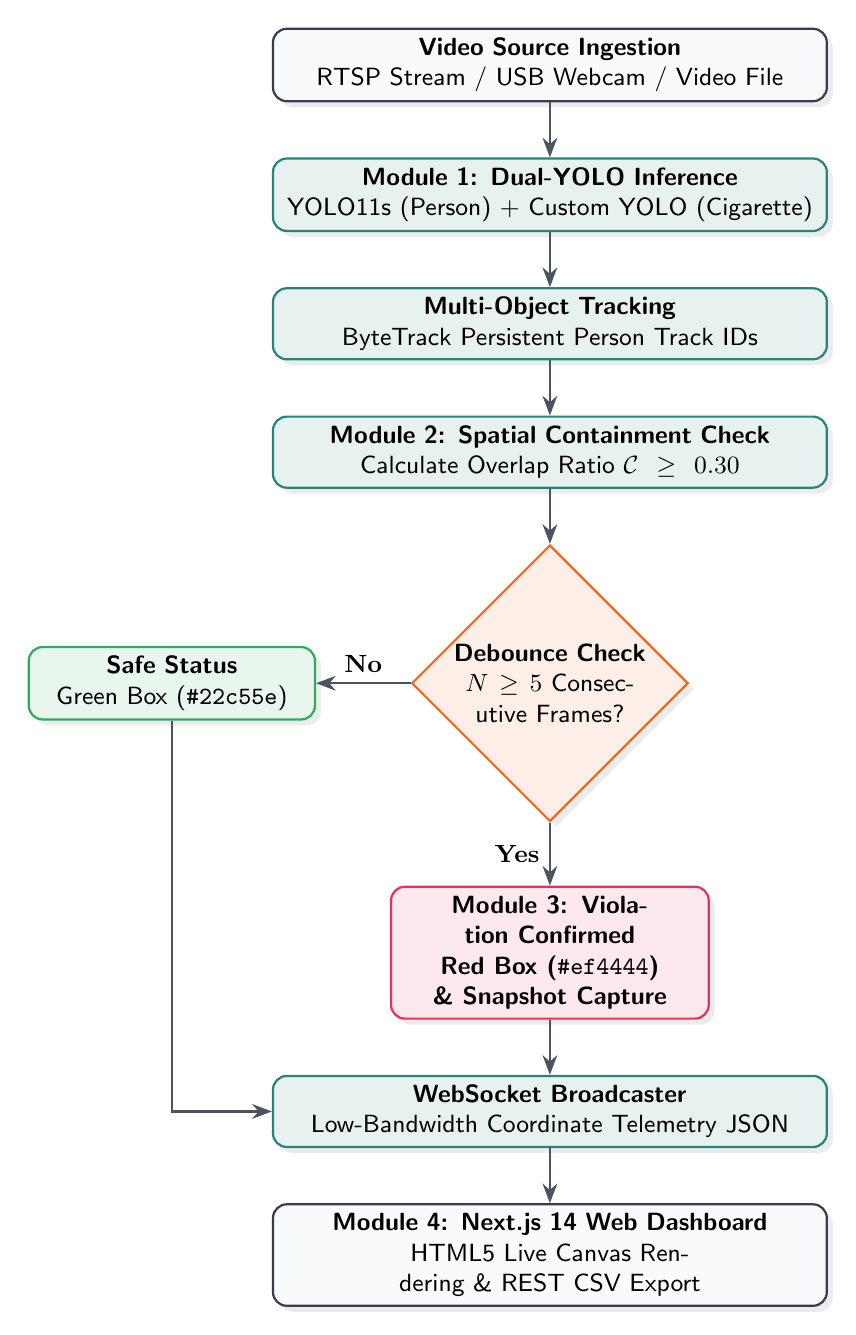
\begin{tikzpicture}[
    node distance=0.7cm,
    auto,
    block/.style={rectangle, draw=primary!90, fill=lightbg, rounded corners=5pt, text width=6.8cm, align=center, minimum height=0.85cm, font=\small\sffamily, thick, drop shadow={opacity=0.15}},
    process/.style={rectangle, draw=secondary!90, fill=secondary!10, rounded corners=5pt, text width=6.8cm, align=center, minimum height=0.85cm, font=\small\sffamily, thick, drop shadow={opacity=0.15}},
    decision/.style={diamond, draw=warning!90, fill=warning!10, text width=2.8cm, align=center, inner sep=-2pt, font=\small\sffamily, thick, drop shadow={opacity=0.15}},
    alert/.style={rectangle, draw=accent!90, fill=accent!10, rounded corners=5pt, text width=3.8cm, align=center, minimum height=0.85cm, font=\small\sffamily\bfseries, thick, drop shadow={opacity=0.15}},
    safe/.style={rectangle, draw=safe!90, fill=safe!10, rounded corners=5pt, text width=3.4cm, align=center, minimum height=0.85cm, font=\small\sffamily, thick, drop shadow={opacity=0.15}},
    line/.style={draw=primary!80, -{Stealth[length=2.5mm]}, thick}
]

    % Nodes
    \node [block] (input) {\textbf{Video Source Ingestion}\\RTSP Stream / USB Webcam / Video File};
    \node [process, below=of input] (yolo) {\textbf{Module 1: Dual-YOLO Inference}\\YOLO11s (Person) + Custom YOLO (Cigarette)};
    \node [process, below=of yolo] (tracking) {\textbf{Multi-Object Tracking}\\ByteTrack Persistent Person Track IDs};
    \node [process, below=of tracking] (containment) {\textbf{Module 2: Spatial Containment Check}\\Calculate Overlap Ratio $\mathcal{C} \ge 0.30$};
    \node [decision, below=of containment] (debounce) {\textbf{Debounce Check}\\$N \ge 5$ Consecutive Frames?};
    
    % Branches
    \node [safe, left=1.2cm of debounce] (safe_state) {\textbf{Safe Status}\\Green Box (\texttt{\#22c55e})};
    \node [alert, below=0.8cm of debounce] (violation_state) {\textbf{Module 3: Violation Confirmed}\\Red Box (\texttt{\#ef4444}) \& Snapshot Capture};
    
    \node [process, below=of violation_state] (ws_pub) {\textbf{WebSocket Broadcaster}\\Low-Bandwidth Coordinate Telemetry JSON};
    \node [block, below=of ws_pub] (frontend) {\textbf{Module 4: Next.js 14 Web Dashboard}\\HTML5 Live Canvas Rendering \& REST CSV Export};

    % Paths
    \path [line] (input) -- (yolo);
    \path [line] (yolo) -- (tracking);
    \path [line] (tracking) -- (containment);
    \path [line] (containment) -- (debounce);
    \path [line] (debounce) -- node[left, font=\small\bfseries] {Yes} (violation_state);
    \path [line] (debounce) -- node[above, font=\small\bfseries] {No} (safe_state);
    \path [line] (safe_state) |- (ws_pub);
    \path [line] (violation_state) -- (ws_pub);
    \path [line] (ws_pub) -- (frontend);

\end{tikzpicture}
\caption{Vertical Operational Flowchart of SmokeGuard AI System Architecture.}
\label{fig:vertical_flowchart}
\end{figure}

\subsection{Modular Subsystem Breakdown}
\begin{enumerate}[leftmargin=*]
    \item \textbf{Module 1 — Dual-Model Detection \& Tracking}: Runs \texttt{yolo11s.pt} and \texttt{best.pt} sequentially on raw frames. ByteTrack anchors persistent person track IDs across frames.
    \item \textbf{Module 2 — Spatial Containment Linking}: Performs pairwise spatial matching between every cigarette box and person box. If containment ratio $\mathcal{C} \ge 0.30$, the cigarette is spatially linked to the person track ID.
    \item \textbf{Module 3 — Evidence Capture \& WebSocket Broadcast}: Triggers snapshot generation and database record creation on state transition to `"violation"`, and broadcasts coordinate telemetry JSON.
    \item \textbf{Module 4 — Reporting \& Retrieval REST API}: Handles client HTTP requests for `/api/violations` listing, `/api/violations/stats` summaries, and `/api/violations/export` downloadable CSV reports.
\end{enumerate}

\subsection{Summary of Design Assumptions}
\begin{itemize}[leftmargin=*]
    \item Person detection and ByteTrack tracking execute prior to cigarette linking in each frame loop.
    \item If a cigarette satisfies the containment threshold for multiple persons, it is assigned to the person with the highest containment ratio.
    \item The violation record closing timestamp (\texttt{ended\_at}) is automatically updated when a tracked person transitions back to `"safe"` status.
\end{itemize}

\section{System Configurations and Hyperparameters}

Preserved default configuration parameters in \texttt{ml/inference/config.py} are presented in Table~\ref{tab:config_params}.

\begin{table}[H]
\centering
\caption{Preserved Inference Hyperparameters and System Thresholds}
\label{tab:config_params}
\small
\vspace{0.4em}
\begin{tabular}{llp{8cm}}
\toprule
\textbf{Parameter} & \textbf{Default Value} & \textbf{Technical Description} \\
\midrule
\texttt{PERSON\_CONF} & \texttt{0.40} & Minimum confidence score threshold for person detection. \\
\texttt{CIG\_CONF} & \texttt{0.25} & Confidence threshold for small-object cigarette detection. \\
\texttt{IOU\_THRESH} & \texttt{0.45} & Non-Maximum Suppression (NMS) IoU threshold. \\
\texttt{OVERLAP\_THRESH} & \texttt{0.30} & Spatial containment ratio ($\text{Area}_{\text{cig inside person}} / \text{Area}_{\text{cig}}$). \\
\texttt{DEBOUNCE\_FRAMES} & \texttt{5} & Required consecutive frames of positive detection to declare a violation. \\
\bottomrule
\end{tabular}
\end{table}

\section{Author Contributions Statement}

\textbf{Tarun Kumar Agnihotri} (Lead Author) conceived the system engineering strategy, developed the complete full-stack codebase, implemented the dual-YOLO model inference pipeline, engineered the spatial containment math and ByteTrack integration, built the FastAPI backend and WebSocket broadcaster, and designed the Next.js live canvas UI. 

\textbf{Arnav Singh} and \textbf{Shubh Jaiswal} (Co-Authors) conducted the background literature review, conducted domain research on small-object detection bottlenecks, analyzed traditional surveillance failures, and formulated the academic research gap analysis.

\section{Conclusion}

SmokeGuard AI successfully addresses the critical operational limitations of traditional smoking detection systems. By combining dual-YOLO inference, ByteTrack multi-object tracking, Spatial Containment mathematics, temporal state debouncing, and decoupled WebSocket telemetry streaming, the platform delivers high accuracy, zero network bandwidth bottlenecks, and complete forensic audit compliance.

\end{document}
